%%% Copyright (C) 2018 Vincent Goulet
%%%
%%% Ce fichier fait partie du projet
%%% «Théorie de la crédibilité avec R»
%%% http://github.com/vigou3/theorie-credibilite-avec-r
%%%
%%% Cette création est mise à disposition selon le contrat
%%% Attribution-Partage dans les mêmes conditions 4.0
%%% International de Creative Commons.
%%% http://creativecommons.org/licenses/by-sa/4.0/

\documentclass[letterpaper,11pt,x11names,english,french]{memoir}
  \usepackage{natbib,url}
  \usepackage{babel}
  \usepackage[autolanguage]{numprint}
  \usepackage{amsmath,amsthm}
  \usepackage[noae]{Sweave}
  \usepackage{graphicx}
  \usepackage{framed}                  % env. snugshade*, oframed
  \usepackage[absolute]{textpos}       % éléments des pages de titre
  \usepackage[shortlabels]{enumitem}   % configuration listes
  \usepackage{multicol}                % environnement multicols
  \usepackage{float}                   % positionnement [H] annexe C
  \usepackage{relsize}                 % \smaller et al.
  \usepackage{manfnt}                  % \mantriangleright (puce)
  \usepackage{metalogo}                % \XeLaTeX logo
  \usepackage{applekeys}               % touches Mac
  \usepackage{dirtree}                 % arbre pour exercice sur \include
  \usepackage{fontawesome}             % icônes \fa*
  \usepackage{awesomebox}              % boites info, important, etc.
  \usepackage{answers}                 % exercices et solutions
  \usepackage{listings}                % code informatique
  \usepackage{pgf}                     % transparence pour couverture avant

  %%% =============================
  %%%  Informations de publication
  %%% =============================
  \title{Théorie de la crédibilité avec R}
  \author{Vincent Goulet}
  \renewcommand{\year}{2018}
  \renewcommand{\month}{01-1}
  \newcommand{\ghurl}{https://github.com/vigou3/theorie-credibilite-avec-r/}

  %%% ===================
  %%%  Style du document
  %%% ===================

  %% Polices de caractères
  \usepackage{fontspec}
  \usepackage{unicode-math}
  \defaultfontfeatures{Scale=0.92}
  \setmainfont[Ligatures=TeX,Numbers=OldStyle]{Lucida Bright OT}
  \setmathfont{Lucida Bright Math OT}
  \setmonofont{Lucida Grande Mono DK}
  \setsansfont[Scale=1.0,Numbers=OldStyle]{Myriad Pro}
  \newfontfamily\fullcaps[Letters=Uppercase,Numbers=Uppercase]{Myriad Pro}
  \usepackage[babel=true]{microtype}
  \usepackage{icomma}

  %% Couleurs
  \usepackage{xcolor}
  \definecolor{comments}{rgb}{0.7,0,0}      % commentaires
  \definecolor{link}{rgb}{0,0.4,0.6}        % liens internes
  \definecolor{url}{rgb}{0.6,0,0}           % liens externes
  \definecolor{citation}{rgb}{0,0.5,0}      % citations
  \definecolor{codebg}{named}{LightYellow1} % fond code R
  \definecolor{prob}{named}{orange}         % encadrés «problème»
  \definecolor{rouge}{rgb}{0.85,0,0.07} % rouge bandeau identitaire
  \definecolor{or}{rgb}{1,0.8,0}        % or bandeau identitaire

  %% Hyperliens
  \usepackage{hyperref}
  \hypersetup{%
    pdfauthor = \theauthor,
    pdftitle = \thetitle,
    colorlinks = true,
    linktocpage = true,
    urlcolor = {url},
    linkcolor = {link},
    citecolor = {citation},
    pdfpagemode = {UseOutlines},
    pdfstartview = {Fit}}
  \setlength{\XeTeXLinkMargin}{1pt}

  %% Affichage de la table des matières du PDF
  \usepackage{bookmark}
  \bookmarksetup{%
    open = true,
    depth = 3,
    numbered = true}

  %% Étiquettes de \autoref (redéfinitions compatibles avec babel).
  %% Attention! Les % à la fin des lignes sont importants sinon des
  %% blancs apparaissent dès que la commande \selectlanguage est
  %% utilisée... comme dans la bibliographie, par exemple.
  \addto\extrasfrench{%
    \def\appendixautorefname{annexe}%
    \def\figureautorefname{figure}%
    \def\exempleautorefname{exemple}%
    \def\exerciceautorefname{exercice}%
    \def\subfigureautorefname{figure}%
    \def\subsectionautorefname{section}%
    \def\subtableautorefname{tableau}%
    \def\tableautorefname{tableau}%
  }

  %% Table des matières (inspirée de classicthesis.sty)
  \renewcommand{\cftchapterleader}{\hspace{1.5em}}
  \renewcommand{\cftchapterafterpnum}{\cftparfillskip}
  \renewcommand{\cftsectionleader}{\hspace{1.5em}}
  \renewcommand{\cftsectionafterpnum}{\cftparfillskip}

  %% Titres des chapitres
  \chapterstyle{hangnum}
  \renewcommand{\chaptitlefont}{\normalfont\Huge\sffamily\bfseries\raggedright}

  %% Marges, entêtes et pieds de page
  \setlength{\marginparsep}{7mm}
  \setlength{\marginparwidth}{13mm}
  \setlength{\headwidth}{\textwidth}
  \addtolength{\headwidth}{\marginparsep}
  \addtolength{\headwidth}{\marginparwidth}

  %% Titres des sections et sous-sections
  \setsecheadstyle{\normalfont\Large\sffamily\bfseries\raggedright}
  \setsubsecheadstyle{\normalfont\large\sffamily\bfseries\raggedright}
  \maxsecnumdepth{subsection}
  \setsecnumdepth{subsection}

  %% Listes. Paramétrage avec enumitem.
  \setlist[enumerate]{leftmargin=*,align=left}
  \setlist[enumerate,2]{label=\alph*),labelsep=*,leftmargin=1.5em}
  \setlist[enumerate,3]{label=\roman*),labelsep=*,leftmargin=1.5em,align=right}
  \setlist[itemize]{leftmargin=*,align=left}

  %% Options de babel
  \frenchbsetup{CompactItemize=false,%
    ThinSpaceInFrenchNumbers=true,
    ItemLabeli=\mantriangleright,
    ItemLabelii=\textendash,
    og=«, fg=»}
  \addto\captionsfrench{\def\figurename{{\scshape Fig.}}}
  \addto\captionsfrench{\def\tablename{{\scshape Tab.}}}

  %%% =========================
  %%%  Sections de code source
  %%% =========================
  \lstloadlanguages{R}
  \lstdefinelanguage{Renhanced}[]{R}{%
    morekeywords={colMeans,colSums,head,is.na,is.null,mapply,ms,na.rm,%
      nlmin,replicate,row.names,rowMeans,rowSums,sys.time,system.time,%
      tail,which.max,which.min,letters,LETTERS},
    deletekeywords={c,start},
    alsoletter={.\%},%
    alsoother={:_\$}}
  \lstset{language=Renhanced,
    extendedchars=true,
    basicstyle=\small\ttfamily\NoAutoSpacing,
    commentstyle=\color{comments}\slshape,
    keywordstyle=\mdseries,
    showstringspaces=false,
    index=[1][keywords],
    indexstyle=\indexcode}

  %%% =========================
  %%%  Nouveaux environnements
  %%% =========================

  %% Environnements d'exemples et al.
  \theoremstyle{remark}
  \newtheorem*{rem}{Remarque}
  \newtheorem*{rems}{Remarques}

  %% Redéfinition de l'environnement titled-frame de framed.sty avec
  %% deux modifications: épaisseur des filets réduite de 2pt à 1pt;
  %% "(suite)" plutôt que "(cont)" dans la barre de titre
  %% lorsque l'encadré se poursuit après un saut de page.
  \renewenvironment{titled-frame}[1]{%
    \def\FrameCommand{\fboxsep8pt\fboxrule1pt
      \TitleBarFrame{\textbf{#1}}}%
    \def\FirstFrameCommand{\fboxsep8pt\fboxrule1pt
      \TitleBarFrame[$\blacktriangleright$]{\textbf{#1}}}%
    \def\MidFrameCommand{\fboxsep8pt\fboxrule1pt
      \TitleBarFrame[$\blacktriangleright$]{\textbf{#1\ (suite)}}}%
    \def\LastFrameCommand{\fboxsep8pt\fboxrule1pt
      \TitleBarFrame{\textbf{#1\ (suite)}}}%
    \MakeFramed{\advance\hsize-16pt \FrameRestore}}%
  {\endMakeFramed}

  %% Encadré générique avec titre basé sur titled-frame, ci-dessus.
  %% Sert pour les listes d'objectifs et les encadrés reliés aux
  %% problèmes (mises en situation) dans les chapitres. Arguments:
  %% couleur du cadre (optionnel; noir par défaut) et titre de la
  %% boite (obligatoire).
  \newenvironment{emphbox}[2][black]{%
    \colorlet{TFFrameColor}{#1}%
    \colorlet{TFTitleColor}{white}%
    \begin{titled-frame}{\sffamily #2}%
      \setlength{\parindent}{0pt}}%
    {\end{titled-frame}}

  %% Liste d'objectifs au début des chapitres
  \newenvironment{objectifs}{%
    \begin{emphbox}{\rule[-7pt]{0pt}{20pt} Objectifs du chapitre}
      \begin{itemize}[nosep]
        \small\sffamily}%
      {\end{itemize}\end{emphbox}}

  %% Problèmes (mises en situation) des chapitres: énoncé au début du
  %% chapitre; astuces en cours de chapitre; solution à la fin
  %% du chapitre.
  \newenvironment{prob-enonce}{%
    \begin{emphbox}[prob]{{\normalfont\faCogs}\; Énoncé du problème}}%
    {\end{emphbox}}
  \newenvironment{prob-astuce}{%
    \begin{emphbox}[prob]{{\normalfont\faBolt}\; Astuce}}%
    {\end{emphbox}}
  \newenvironment{prob-solution}{%
    \begin{emphbox}[prob]{{\normalfont\faLightbulbO}\; Solution du problème}}%
    {\end{emphbox}}

  %% Environnements de Sweave. Les environnements Sinput et Soutput
  %% utilisent Verbatim (de fancyvrb). On les réinitialise pour
  %% enlever la configuration par défaut de Sweave, puis on réduit
  %% l'écart entre les blocs Sinput et Soutput.
  \DefineVerbatimEnvironment{Sinput}{Verbatim}{}
  \DefineVerbatimEnvironment{Soutput}{Verbatim}{}
  \fvset{listparameters={\setlength{\topsep}{0pt}}}

  %% L'environnement Schunk est complètement redéfini en un hybride
  %% des environnements snugshade* et leftbar de framed.sty.
  \makeatletter
  \renewenvironment{Schunk}{%
    \setlength{\topsep}{1pt}
    \def\FrameCommand##1{\hskip\@totalleftmargin
       \vrule width 2pt\colorbox{codebg}{\hspace{3pt}##1}%
      % There is no \@totalrightmargin, so:
      \hskip-\linewidth \hskip-\@totalleftmargin \hskip\columnwidth}%
    \MakeFramed {\advance\hsize-\width
      \@totalleftmargin\z@ \linewidth\hsize
      \advance\labelsep\fboxsep
      \@setminipage}%
  }{\par\unskip\@minipagefalse\endMakeFramed}
  \makeatother

  %% Exercices et réponses
  \Newassociation{sol}{solution}{solutions}
  \newcounter{exercice}[chapter]
  \renewcommand{\theexercice}{\thechapter.\arabic{exercice}}
  \newenvironment{exercice}[1][]{%
    \begin{list}{}{%
        \refstepcounter{exercice}
        \ifthenelse{\equal{#1}{nosol}}{%
          \renewcommand{\makelabel}{\bfseries\theexercice}}{%
          \hypertarget{ex:\theexercice}{}
          \Writetofile{solutions}{\protect\hypertarget{sol:\theexercice}{}}
          \renewcommand{\makelabel}{%
            \bfseries\protect\hyperlink{sol:\theexercice}{\theexercice}}}
        \settowidth{\labelwidth}{\bfseries\theexercice}
        \setlength{\leftmargin}{\labelwidth}
        \addtolength{\leftmargin}{\labelsep}
        \setlist[enumerate,1]{label=\alph*),labelsep=*,leftmargin=1.5em}
        \setlist[enumerate,2]{label=\roman*),labelsep=0.5em,align=right}}
      \item}%
      {\end{list}}
  \renewenvironment{solution}[1]{%
    \begin{list}{}{%
        \renewcommand{\makelabel}{%
          \bfseries\protect\hyperlink{ex:#1}{#1}}
        \settowidth{\labelwidth}{\bfseries #1}
        \setlength{\leftmargin}{\labelwidth}
        \addtolength{\leftmargin}{\labelsep}
        \setlist[enumerate,1]{label=\alph*),labelsep=*,leftmargin=1.5em}
        \setlist[enumerate,2]{label=\roman*),labelsep=0.5em,align=right}}
      \item}
    {\end{list}}

  %% Listes de commandes
  \newenvironment{ttscript}[1]{%
    \begin{list}{}{%
        \setlength{\labelsep}{1.5ex}
        \settowidth{\labelwidth}{\fbox{#1}}
        \setlength{\leftmargin}{\labelwidth}
        \addtolength{\leftmargin}{\labelsep}
        \setlength{\parsep}{0.5ex plus0.2ex minus0.2ex}
        \setlength{\itemsep}{0.3ex}
        \renewcommand{\makelabel}[1]{\vphantom{|}##1\hfill}}}
    {\end{list}}

  %%% =====================
  %%%  Nouvelles commandes
  %%% =====================

  %% Noms de fonctions, code, etc.
  \newcommand{\code}[1]{\texttt{#1}}
  \newcommand{\pkg}[1]{\textbf{#1}}

  %% Hyperlien avec symbole de lien externe juste après; second
  %% argument peut être vide pour afficher l'url comme lien
  %% [https://tex.stackexchange.com/q/53068/24355 pour procédure de
  %% test du second paramètre vide]
  \newcommand{\link}[2]{%
    \def\param{#2}%
    \ifx\param\empty
      \href{#1}{\nolinkurl{#1}~\raisebox{-0.1ex}{\smaller\faExternalLink}}%
    \else
      \href{#1}{#2~\raisebox{-0.1ex}{\smaller\faExternalLink}}%
    \fi
  }

  %% Indications de capsule vidéo
  \newcommand{\capsule}[2]{\href{#1}{#2}\marginpar{%
      \href{#1}{\raisebox{-0.5em}[0em][0em]{\Huge\faYoutubePlay}}}}

  %% Boites additionnelles (basées sur awesomebox.sty) pour remarques
  %% spécifiques à macOS et Windows
  \newcommand{\osxbox}[1]{%
    \awesomebox{\faApple}{\aweboxrulewidth}{black}{#1}}
  \newcommand{\windowsbox}[1]{%
    \awesomebox{\faWindows}{\aweboxrulewidth}{black}{#1}}

  %% Boite pour le nom du fichier de script correspondant au début des
  %% sections d'exemples.
  \newcommand{\scriptfile}[1]{%
    \begingroup
    \noindent
    \mbox{%
      \makebox[3mm][l]{\raisebox{-0.5pt}{\small\faChevronCircleDown}}\;%
      \smaller[1] {\sffamily Fichier d'accompagnement} {\ttfamily #1}}
    \endgroup}

  %% Lien vers GitHub dans la page de notices
  \newcommand{\viewsource}[1]{%
    \href{#1}{%
      Voir sur GitHub \raisebox{-1pt}{\footnotesize\faGithub}}}

  %% «Logo» C++
  \newcommand{\Rplus}{\protect\hspace{-.05em}\protect\raisebox{.2ex}{\smaller\textbf{+}}}
  \newcommand{\Cpp}{\mbox{C\Rplus\Rplus}\xspace}

  %% Raccourcis usuels vg
  \newcommand{\pt}{{\scriptscriptstyle \Sigma}}
  \newcommand{\mat}[1]{\mathbf{#1}}
  \newcommand{\var}[1]{\operatorname{Var} [ #1 ]}

  %%% =======
  %%%  Index
  %%% =======
  \newcommand{\bfhyperpage}[1]{\textbf{\hyperpage{#1}}}
  \renewcommand{\preindexhook}{%
    Les numéros de page en caractères gras indiquent les pages où les
    concepts sont introduits, définis ou expliqués.\vskip\onelineskip}
  \newcommand{\Index}[1]{\index{#1|bfhyperpage}}
  \newcommand{\indexcode}[1]{\index{#1@\code{#1}}}
  \newcommand{\Indexcode}[1]{\Index{#1@\code{#1}}}
  \newcommand{\icode}[1]{\indexcode{#1}\code{#1}}
  \newcommand{\Icode}[1]{\Indexcode{#1}\code{#1}}
  \makeindex

  %%% =======
  %%%  Varia
  %%% =======

  %%% Sous-figures
  \newsubfloat{figure}

  %%% Style de la bibliographie
  \bibliographystyle{francais}

  %% Longueurs pour la composition des pages couvertures avant et
  %% arrière.
  \newlength{\banderougewidth} \newlength{\banderougeheight}
  \newlength{\bandeorwidth}    \newlength{\bandeorheight}
  \newlength{\imageheight}
  \newlength{\logoheight}
  \newlength{\gapwidth}

  %% Aide pour la césure
  \hyphenation{%
    con-nai-tre
    con-sole
    cons-tante
    con-tenu
    con-trôle
    nom-bre
    puis-que
  }

%  \includeonly{}

\begin{document}

\frontmatter

\pagestyle{empty}

%%% Copyright (C) 2018 Vincent Goulet
%%%
%%% Ce fichier fait partie du projet
%%% «Théorie de la crédibilité avec R»
%%% http://github.com/vigou3/theorie-credibilite-avec-r
%%%
%%% Cette création est mise à disposition selon le contrat
%%% Attribution-Partage dans les mêmes conditions 4.0
%%% International de Creative Commons.
%%% http://creativecommons.org/licenses/by-sa/4.0/

%%%
%%% Page de titre
%%%

\begingroup
\TPGrid{3}{36}
\textblockorigin{0mm}{0mm}
\setlength{\parindent}{0mm}
\setlength{\imageheight}{29\TPVertModule}
\setlength{\banderougewidth}{2\TPHorizModule}
\setlength{\banderougeheight}{\TPVertModule}
\setlength{\bandeorwidth}{\TPHorizModule}
\setlength{\bandeorheight}{\banderougeheight}
\setlength{\logoheight}{2.5\TPVertModule}
\setlength{\gapwidth}{1.5pt}
\addtolength{\bandeorwidth}{-\gapwidth}
\addtolength{\imageheight}{-\gapwidth}
\setlength{\fboxrule}{3pt}
\setlength{\fboxsep}{0pt}

\def\titlefmt{%
  \sffamily\bfseries\fontsize{45}{45}\selectfont\thetitle\par}
\def\authorfmt{%
  \sffamily\mdseries\fontsize{28}{28}\selectfont\theauthor}
\def\affiliation{%
  \sffamily\mdseries\fontsize{18}{28}\selectfont
  Professeur titulaire \\
  École d'actuariat, Université Laval}
\def\edition{%
  \sffamily\mdseries\fontsize{18}{18}\selectfont
  Édition {\fullcaps\year}.\month}

%% bandeau identitaire
\begin{textblock*}{\paperwidth}[0,1](0mm,30\TPVertModule)
  \textcolor{rouge}{\rule{\banderougewidth}{\banderougeheight}}% % bande rouge
  \rule{\gapwidth}{0pt}%                                         % filet
  \textcolor{or}{\rule{\bandeorwidth}{\bandeorheight}}           % bande or
\end{textblock*}

%% logo UL
\begin{textblock*}{\TPHorizModule}(2\TPHorizModule,31\TPVertModule)
  \rule{\gapwidth}{0pt}%                                         % filet
  
\includegraphics[height=\logoheight,%
                   keepaspectratio=true]{ul_p}
\end{textblock*}

%% image de fond
\begin{textblock*}{\paperwidth}(0mm,0mm)
  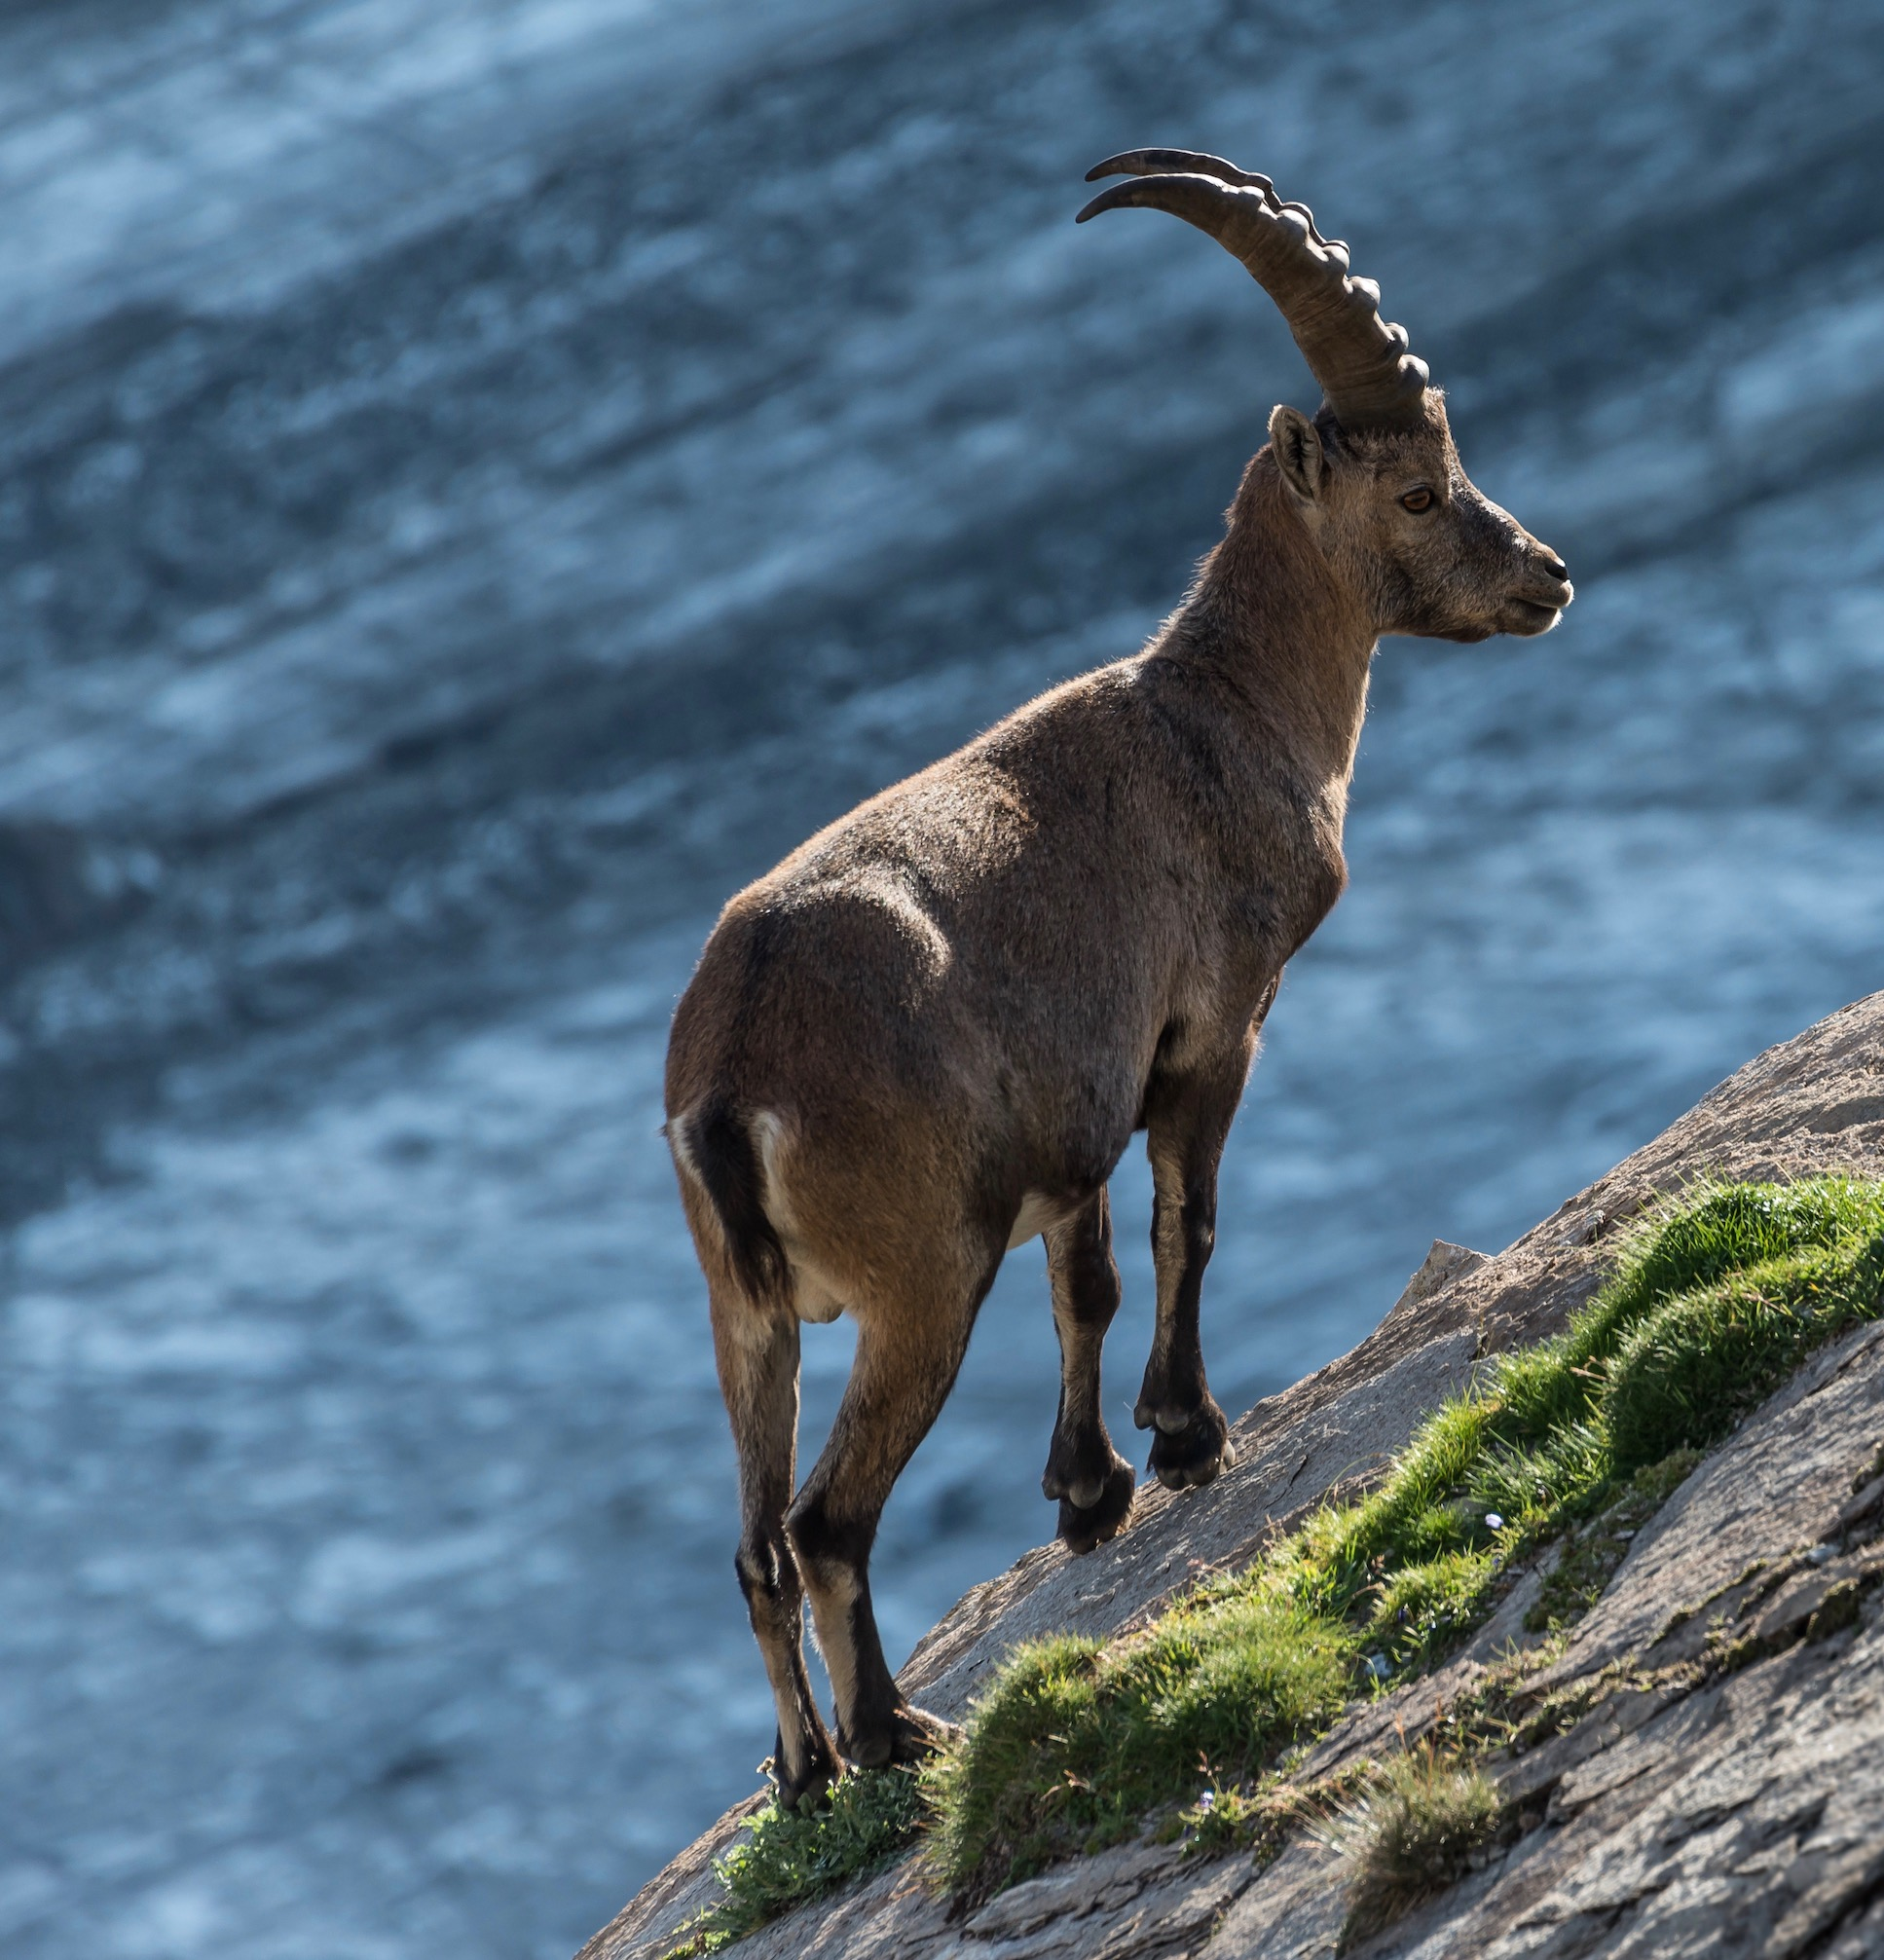
\includegraphics[width=\paperwidth,%
                   keepaspectratio=true]{Steinbock}
\end{textblock*}

%% titre
\begin{textblock*}{2.3\TPHorizModule}(0.35\TPHorizModule,3.5\TPVertModule)
  \pgfsetfillopacity{0.85}
  \textcolor{white}{\titlefmt}
  \pgfsetfillopacity{1}
\end{textblock*}

%% auteur
\begin{textblock*}{2\TPHorizModule}(0.35\TPHorizModule,8.5\TPVertModule)
  \pgfsetfillopacity{0.85}
  \textcolor{white}{\authorfmt}
  \pgfsetfillopacity{1}
\end{textblock*}

\null\cleardoublepage

%%%
%%% Page frontispice
%%%

%% titre
\begin{textblock*}{2.3\TPHorizModule}(0.35\TPHorizModule,3.5\TPVertModule)
  \pgfsetfillopacity{1}       % autrement titre un peu trop haut (?)
  \titlefmt
\end{textblock*}

%% auteur
\begin{textblock*}{2\TPHorizModule}(0.35\TPHorizModule,8.5\TPVertModule)
  \pgfsetfillopacity{1}       % idem
  \authorfmt
\end{textblock*}

%% affiliation
\begin{textblock*}{2\TPHorizModule}(0.35\TPHorizModule,10.5\TPVertModule)
  \affiliation
\end{textblock*}

%% édition
\begin{textblock*}{1.7\TPHorizModule}(0.35\TPHorizModule,30\TPVertModule)
  \edition
\end{textblock*}
\endgroup

%%% Local Variables:
%%% mode: latex
%%% TeX-engine: xetex
%%% TeX-master: "theorie-credibilite-avec-r"
%%% coding: utf-8
%%% End:

\null\cleardoublepage           % cf. section 2.2 textpos.pdf

%%% Copyright (C) 2018 Vincent Goulet
%%%
%%% Ce fichier fait partie du projet
%%% «Théorie de la crédibilité avec R»
%%% http://github.com/vigou3/theorie-credibilite-avec-r
%%%
%%% Cette création est mise à disposition selon le contrat
%%% Attribution-Partage dans les mêmes conditions 4.0
%%% International de Creative Commons.
%%% http://creativecommons.org/licenses/by-sa/4.0/

\begingroup
\calccentering{\unitlength}
\begin{adjustwidth*}{\unitlength}{-\unitlength}
  \setlength{\parindent}{0pt}
  \setlength{\parskip}{\baselineskip}
  \small

  {\textcopyright} {\year} Vincent Goulet \\

  
\includegraphics[height=7mm,keepaspectratio=true]{by-sa}\\%
  Cette création est mise à disposition selon le contrat
  \href{http://creativecommons.org/licenses/by-sa/4.0/deed.fr}{%
    Attribution-Partage dans les mêmes conditions 4.0 International} de
  Creative Commons. En vertu de ce contrat, vous êtes libre de:
  \begin{itemize}
  \item \textbf{partager} --- reproduire, distribuer et communiquer
    l'{\oe}uvre;
  \item \textbf{remixer} --- adapter l'{\oe}uvre;
  \item utiliser cette {\oe}uvre à des fins commerciales.
  \end{itemize}
  Selon les conditions suivantes:

  \begin{tabularx}{\linewidth}{@{}lX@{}}
    \raisebox{-9mm}[0mm][13mm]{%
      
\includegraphics[height=11mm,keepaspectratio=true]{by}} &
    \textbf{Attribution} --- Vous devez créditer l'{\oe}uvre, intégrer
    un lien vers le contrat et indiquer si des modifications ont été
    effectuées à l'{\oe}uvre. Vous devez indiquer ces informations par
    tous les moyens possibles, mais vous ne pouvez suggérer que
    l'Offrant vous soutient ou soutient la façon dont vous avez utilisé
    son {\oe}uvre. \\
    \raisebox{-9mm}{
\includegraphics[height=11mm,keepaspectratio=true]{sa}}
    & \textbf{Partage dans les mêmes conditions} --- Dans le cas où vous
    modifiez, transformez ou créez à partir du matériel composant
    l'{\oe}uvre originale, vous devez diffuser l'{\oe}uvre modifiée dans
    les même conditions, c'est à dire avec le même contrat avec lequel
    l'{\oe}uvre originale a été diffusée.
  \end{tabularx}

  Les exercices sont dérivés de \citet{Cossette:credibilite:2008}, un
  document sous contrat
  \href{http://creativecommons.org/licenses/by-sa/2.5/ca/}{%
    CC BY-SA 2.5 Canada}.

  \textbf{Code source} \\
  \viewsource{\ghurl}

  \textbf{Couverture} \\
  Bouquetin des Alpes (\emph{Capra ibex}) du parc national autrichien du Hohe Tauern.
  Photo: {\textcopyright} Bernd Thaller,
  \href{https://creativecommons.org/licenses/by-sa/3.0/at/deed.en}{CC
    BY-SA 3.0 Autriche}, via
  \href{https://commons.wikimedia.org/w/index.php?curid=40071439}{Wikimedia
    Commons}.
\end{adjustwidth*}
\endgroup

%%% Local Variables:
%%% mode: latex
%%% TeX-engine: xetex
%%% TeX-master: "theorie-credibilite-avec-r"
%%% coding: utf-8
%%% End:

\clearpage

\pagestyle{companion}

%%%% Copyright (C) 2018 Vincent Goulet
%%%
%%% Ce fichier fait partie du projet
%%% «Théorie de la crédibilité avec R»
%%% http://github.com/vigou3/theorie-credibilite-avec-r
%%%
%%% Cette création est mise à disposition selon le contrat
%%% Attribution-Partage dans les mêmes conditions 4.0
%%% International de Creative Commons.
%%% http://creativecommons.org/licenses/by-sa/4.0/

\chapter{Introduction}
\label{chap:introduction}

\tableofcontents*

%% Vignette tirée de xkcd.com
% \cleartoverso
% \thispagestyle{empty}
% \begin{vplace}[0.45]
%   \centering
%   \begin{minipage}{0.9\linewidth}
%     \setkeys{Gin}{width=\textwidth}
%     \includegraphics{images/compiling.png} \\
%     \footnotesize\sffamily%
%     Tiré de \href{http://xkcd.com/303/}{XKCD.com}
%   \end{minipage}
% \end{vplace}

\mainmatter

%\include{}

\appendix
%\chapter{Solutions}
\label{chap:solutions}

\input{solutions-stabilite}
\input{solutions-bayesienne}
\input{solutions-buhlmann}
\input{solutions-buhlmann-straub}

%%% Local Variables:
%%% TeX-master: "theorie-credibilite-avec-r"
%%% TeX-engine: xetex
%%% coding: utf-8
%%% End:


\bibliography{r,stat,informatique,vg}

\cleardoublepage
\printindex

\pagestyle{empty}

\cleartoverso
%%% Copyright (C) 2018 Vincent Goulet
%%%
%%% Ce fichier fait partie du projet
%%% «Théorie de la crédibilité avec R»
%%% http://github.com/vigou3/theorie-credibilite-avec-r
%%%
%%% Cette création est mise à disposition selon le contrat
%%% Attribution-Partage dans les mêmes conditions 4.0
%%% International de Creative Commons.
%%% http://creativecommons.org/licenses/by-sa/4.0/

\vspace*{\fill}

\begingroup
\calccentering{\unitlength}
\begin{adjustwidth*}{\unitlength}{-\unitlength}
  \begin{flushleft}
    \small %
    Ce document a été produit avec le système de mise en page
    {\XeLaTeX}. Le texte principal est en Lucida Bright~OT 11~points,
    les mathématiques en Lucida Bright Math~OT, le code informatique
    en Lucida Grande Mono~DK et les titres en Adobe Myriad~Pro. Des
    icônes proviennent de la police Font~Awesome. Les graphiques ont
    été réalisés avec R.
  \end{flushleft}
\end{adjustwidth*}
\endgroup
\vfill


\cleartoverso
%%% Copyright (C) 2018 Vincent Goulet
%%%
%%% Ce fichier fait partie du projet
%%% «Théorie de la crédibilité avec R»
%%% http://github.com/vigou3/theorie-credibilite-avec-r
%%%
%%% Cette création est mise à disposition selon le contrat
%%% Attribution-Partage dans les mêmes conditions 4.0
%%% International de Creative Commons.
%%% http://creativecommons.org/licenses/by-sa/4.0/

\begingroup

\TPGrid{3}{36}
\textblockorigin{0mm}{0mm}
\setlength{\parindent}{0mm}
\setlength{\banderougewidth}{2\TPHorizModule}
\setlength{\bandeorwidth}{\TPHorizModule}
\setlength{\gapwidth}{2pt}
\addtolength{\bandeorwidth}{-\gapwidth}

%% bandeau identitaire arrière
\begin{textblock*}{8.5in}[0,1](0mm,30\TPVertModule)
  \textcolor{or}{\rule{\bandeorwidth}{\TPVertModule}}%      % bande or
  \rule{\gapwidth}{0pt}%                                    % filet
  \textcolor{rouge}{\rule{\banderougewidth}{\TPVertModule}} % bande rouge
\end{textblock*}

% code-barre
\begin{textblock*}{0.9\TPHorizModule}(0.1\TPHorizModule,25\TPVertModule)
  % \includegraphics[height=4\TPVertModule]{codebarre_\ISBN}
\end{textblock*}

\endgroup

%%% Local Variables:
%%% mode: latex
%%% TeX-engine: xetex
%%% TeX-master: "theorie-credibilite-avec-r"
%%% coding: utf-8
%%% End:


\end{document}

%%% Local Variables:
%%% mode: latex
%%% TeX-engine: xetex
%%% TeX-master: t
%%% coding: utf-8
%%% End:
